\chapter{Intelligent History}
\label{ch:Intelligent-History}

To enable the investigation of our hypothesis, we developed Intelligent History,\footnote{\url{https://github.com/Alison-Li/intelligent-history}, verified 5/22/2022.} 
a prototype plugin for the IntelliJ IDEA \entity{IDE}.
We describe the design goals of the approach that motivated the development of Intelligent History in \autoref{sec:Design-Goals}. 
In \autoref{sec:Implementation}, we demonstrate how these design principles were realized in the implementation of Intelligent History. 
We elaborate on the heuristics Intelligent History uses for suggesting more meaningful comments in \autoref{sec:Heuristics}.
Finally, we walk through an example in \autoref{sec:Use-Case} to illustrate how Intelligent History can be used for obtaining code rationale information effectively from a file's revision history.

%%%%%%%%%%%%%%%%%%%%%%%%%%%%%%%%%%%%%%%%%%%%%%%%%%%%%%%%%%%%%%%%%%%%%%
\section{Design Goals}
\label{sec:Design-Goals}

As Codoban \etal observed in their study, the high volume of changes presented in the commit history 
for a software project results in cognitive load for developers \cite{codoban_software_2015}.
The study found that developers manually employed various strategies that would 
reduce the number of commits they needed to closely analyze.
To reduce the number of commits, developers may recall a date range in which 
a change was made and only examine commits from the date range.
Developers also filter commits based on certain keywords and skim the diffs 
in commits to look for only the commits that are relevant to their current task.
Combined with the strategy of reducing the search space of commits, 
developers further describe iterating through past versions of a file to find when specific functionality was implemented.
\rev{The need to navigate a sizable quantiy of commits in a revision history} 
makes locating information about the rationale for how a change affected a code segment, 
the broader modification a change was part of, 
and how the code segment interacted with surrounding code at a specific point in time more challenging.

\rev{Additionally, developers demonstrate a need for more convenient access
to information that can reveal the context and motivation behind code.
Issues from issue tracking systems have been utilized as a source of
code rationale information in previous work \cite{rastkar_why_2013,moreno_arena_2017,bradley_supporting_2011},
Implemented as Eclipse \entity{IDE} plugins, Bradley and Murphy compared two user interfaces 
for exploring software history that both integrated issue information
from Bugzilla to help contextualize revision history \cite{bradley_supporting_2011}.
From their study evaluating the interfaces with 11 participants, Bradley and Murphy report a general enthusiasm for
an integrated view of rationale information and source code.}

The design of our approach in Intelligent History is guided by two goals: 

\begin{enumerate}[label={(\arabic*)}]
    \item Developers need an approach that can automatically distinguish potentially meaningful commits from less important commits;
    \item Developers need better access to code rationale information when examining commits and explicitly referenced issues.
\end{enumerate}

To achieve (1), we propose an approach to automatically reduce the number of commits a developer must inspect to obtain code rationale information (\autoref{subsec:Reducing-Commit-Search-Space}).
To address (2), we \rev{propose an approach to} integrating the contextual information for source code within the \entity{IDE} that the developer uses (\autoref{subsec:Minimize-Commit-Issue-Distance}).

\subsection{Reducing the Search Space of Commits}
\label{subsec:Reducing-Commit-Search-Space}

We propose \rev{an approach} to relieve cognitive load for developers by automatically reducing the search space of commits.
Our \rev{approach} involves analyzing the diffs between commits in a file's commit history to determine which commits may be less significant in terms of the lines of code changed in the diff.
We convey the outcome of this analysis visually to the developer by applying highlighting on a file's revision history, 
colouring less important commits with a background colour and allowing the remaining commits to appear more prominently in the foreground.
Diffs that solely contain changes, such as white spaces and line-endings, are inefficient for a developer sifting through several commits in a commit history \cite{codoban_software_2015}.
We highlight the commits that have a diff containing code changes beyond a set of non-important changes and fade the other less important commits into the background.
We retain all commits in the file history to increase the confidence of the developer in our approach.
The entire history remains visible for the developer to browse 
and the developer can interpret the highlighting as a suggestion for which commits to prioritize in their information search.

In particular, \emph{tangled changes} pose an obstacle to efficient software revision history exploration 
and is a significant source of noise in commit histories \cite{herzig_tangled_2013}.
Tangled changes refer to a set of changes for two or more separate tasks. 
Murphy-Hill \etal \cite{murphy-hill_refactor_2012} found refactorings are often committed with changes for separate tasks. 
From a study of five open-source Java projects, Herzig and Zeller \cite{herzig_tangled_2013} revealed up to 15\% of all bug fixes to consist of tangled changes and, 
on average, at least 16.5\% of all source files are incorrectly associated with bug reports. 
\rev{54\% of survey respondents from the study by Codoban \etal reported tangled changes to be a problem
in understanding commit history \cite{codoban_software_2015}.}
To simplify the determination of a non-important commit, we have chosen to implement Intelligent History to operate on
the diffs for individual files to identify whether a commit is less important when considering the changes made to a specifc file. 
For example, a commit $c$ that is present in the history for a single file $F$ may have modified multiple other files, 
and be present in the commit history for other files, but to the extent that $F$ is concerned, 
$c$ may have only added a newline at the end of a file.
Thus, $c$ would be identified as trivial for $F$ and would be presented as a faded commit in $F$'s file revision history.

The identification of less important commits in Intelligent History is based on heuristics.
Under Kawrykow and Robillard's definition of a \emph{non-essential} change being cosmetic in nature, 
generally behaviour-preserving, and unlikely to provide further insight into the roles or relationships of program elements \cite{kawrykow_non-essential_2011}, 
we devise four categories of changes to use for identifying less important commits based their diff content.
Specific to the Java programming language, we regard a commit as less important if the changed lines in a commit's diff contains only changes related to: 
\emph{documentation}, \emph{annotations}, \emph{newlines}, and \emph{import} statements.
These heuristics are conservative to mitigate false positives in terms of a non-important change and to maintain generalizability across projects.
We categorize the changed lines in a diff by applying regular expression matching of patterns on each line.
The details of how Intelligent History uses heuristics to determine trivial commits are discussed further in \autoref{sec:Heuristics}.

\subsection{Minimizing the Distance Between Commits and Issues}
\label{subsec:Minimize-Commit-Issue-Distance}

Several studies confirm developers look through change histories and associated issue 
or bug reports for hints about code implementation and rationale \cite{ko_information_2007,robillard_turnover-induced_2021, rastkar_why_2013}.
The issues in issue repositories is a valuable source that current members 
of a project can use for obtaining rationale information as it contains past discussions about design aspects \cite{brunet_design_2014,hassan_road_2008}.
Issues from an issue tracking system (\entity{ITS}) typically contain a title, description, administrative metadata, such as the status of an issue, priority, 
and \rev{comments by developers discussing various aspects of the issue}.
\rev{The comments for an issue provide} insight into technical details 
and opinions that enrich code changes involved in a task with the ``why'' of 
certain design choices in those changes \cite{ortu_jira_2015}.

Some software projects have adopted a convention of adding a prefix referencing 
\rev{the issue associated with a change} in a commit's subject message \cite{rastkar_why_2013,moreno_arena_2017}.
Although the practice of explicitly linking each commit to an issue is helpful when looking for relevant issues from an \entity{ITS}, the developer still experiences cognitive load from switching between their \entity{IDE} and browser when reading and synthesizing the information from several issues.
A software developer examining several issues related to several commits also must maintain a mental model that interleaves the contextual information discovered from issues with code changes in diffs.
\autoref{fig:Cognitive-Load} demonstrates how the distributed nature of commits and issue information can result in cognitive load for a developer browsing the commit history for a file, while also synthesizing the information gained from checking issues related to commits in a separate application.

\begin{figure}
    \center
    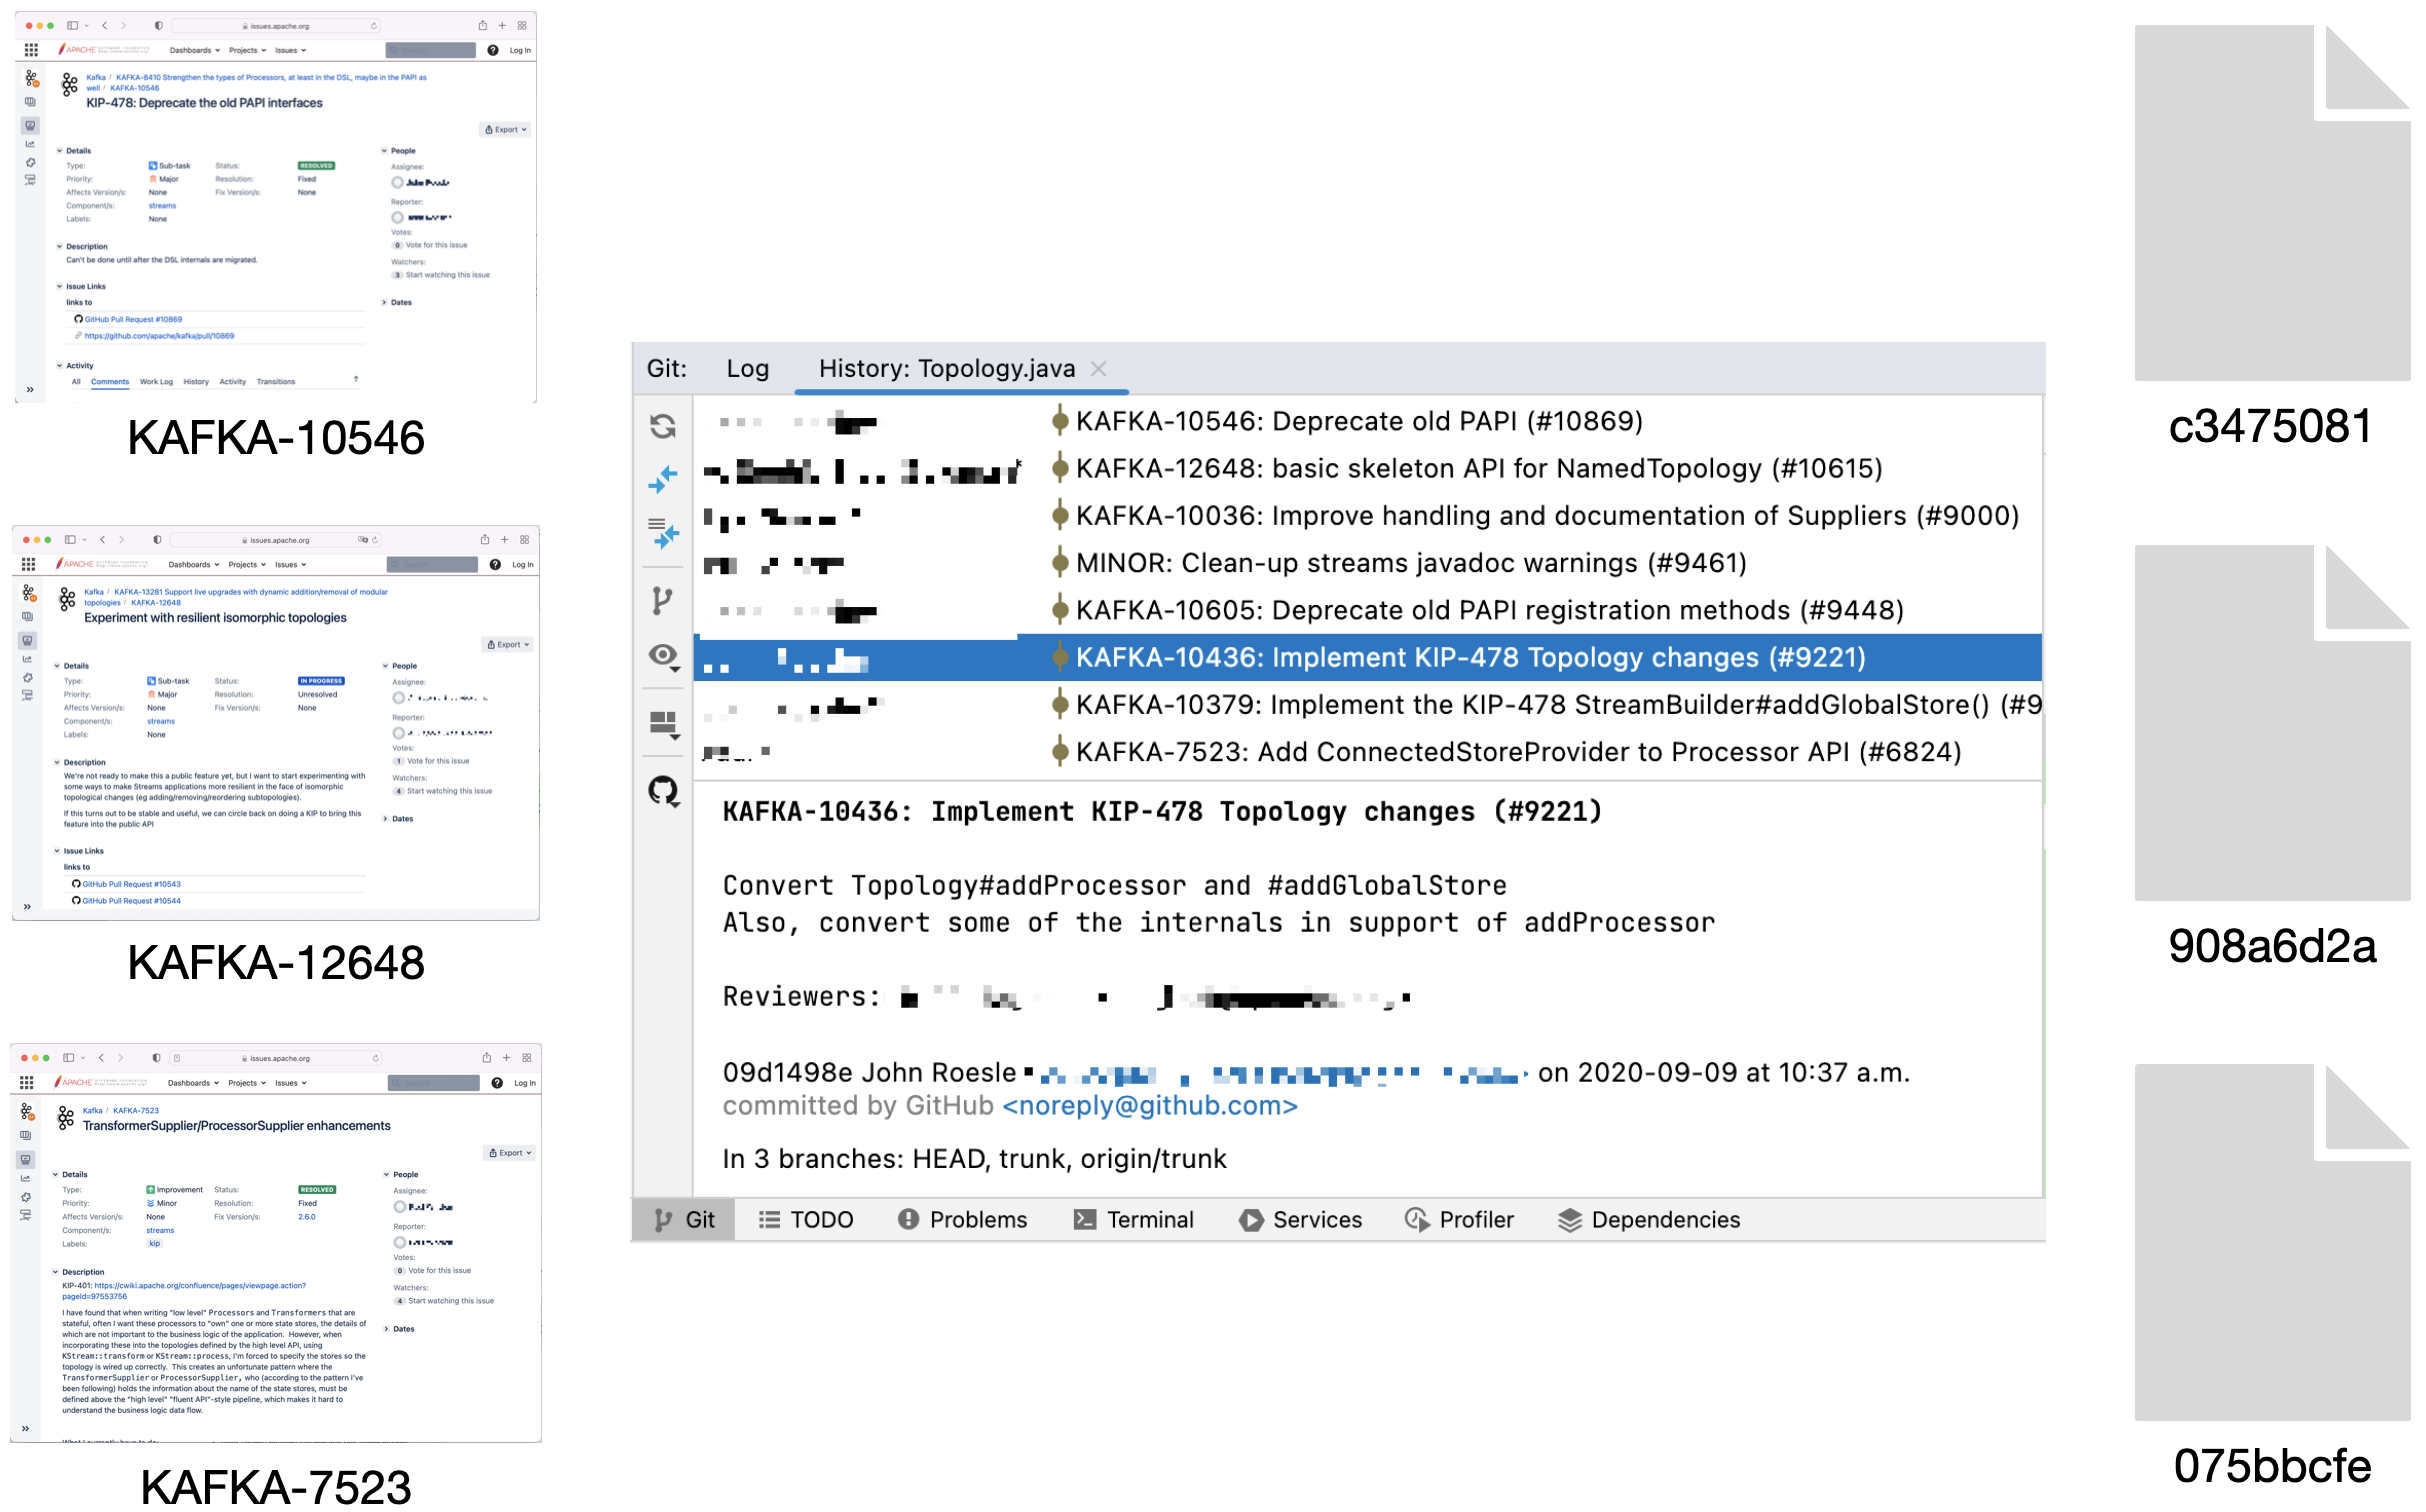
\includegraphics[width=\textwidth]{./images/cognitive-load.png}
    \caption{
        Three Jira issues opened in individual browser windows (left), corresponding to three commits in the file commit history (centre) of the \code{Topology} class in Apache Kafka. 
        The diffs of each commit (right) must also be maintained in the developer's mental model of the changes in history. 
        Illustrates the distributed nature of code change and rationale information between the \entity{IDE} and browser.
    }
    \label{fig:Cognitive-Load}
\end{figure}

In some cases, an issue may not contain any discussion at all or the description in an issue may either be missing 
or too vague to yield any insight on a specific code change or the evolution of code changes in a file.
Thus, in the design of Intelligent History, we found it crucial to co-present commits with issue information in the \entity{IDE}.
\rev{Developers also face information overload from the presentation of issues and 
various metadata about issues from an \entity{ITS} \cite{baysal_issue-overload_2014,bertram_social-nature_2010}.
We propose to compute a subset of information from issues as metadata and display relevant metadata
alongside issues to the developer that could potentially signal to a developer whether a commit's associated issue
may contain any meaningful rationale information. For instance, a higher number of comments on an issue that have been
posted by the commit's author may prompt a developer to further investigate the Jira issue to check if the
commit author left behind any rationale information about the change in their comments.
We describe all of the metrics we compute as part of an issue's metadata in \autoref{sec:Implementation}.}

%%%%%%%%%%%%%%%%%%%%%%%%%%%%%%%%%%%%%%%%%%%%%%%%%%%%%%%%%%%%%%%%%%%%%%
\section{The Intelligent History Plugin}
\label{sec:Implementation}

As part of the effort to reduce the cognitive and temporal costs of software history exploration, 
we chose to develop a plugin to augment the existing rich features an \entity{IDE} already provides.
Unlike a stand-alone desktop or web application, a plugin minimizes the number of external application windows a developer needs to maintain and explore to gain context around revisions. 
This is because the information Intelligent History offers \rev{is} integrated within the \entity{IDE}, 
reducing the number of switches a developer has to perform between a separate browser window for searching an issue tracking system (\entity{ITS})
and their \entity{IDE} for examining source code and revision history.
IntelliJ provides a built-in Git client \entity{GUI} for navigating a software project's revision history and inspecting revisions. 
In particular, the ``Show History'' feature in IntelliJ is available for directories and files, 
and displays a history of commits that affected a single file or directory.
\autoref{fig:IntelliJ-Overview} shows IntelliJ with a file's commit history visible.

\begin{figure}
    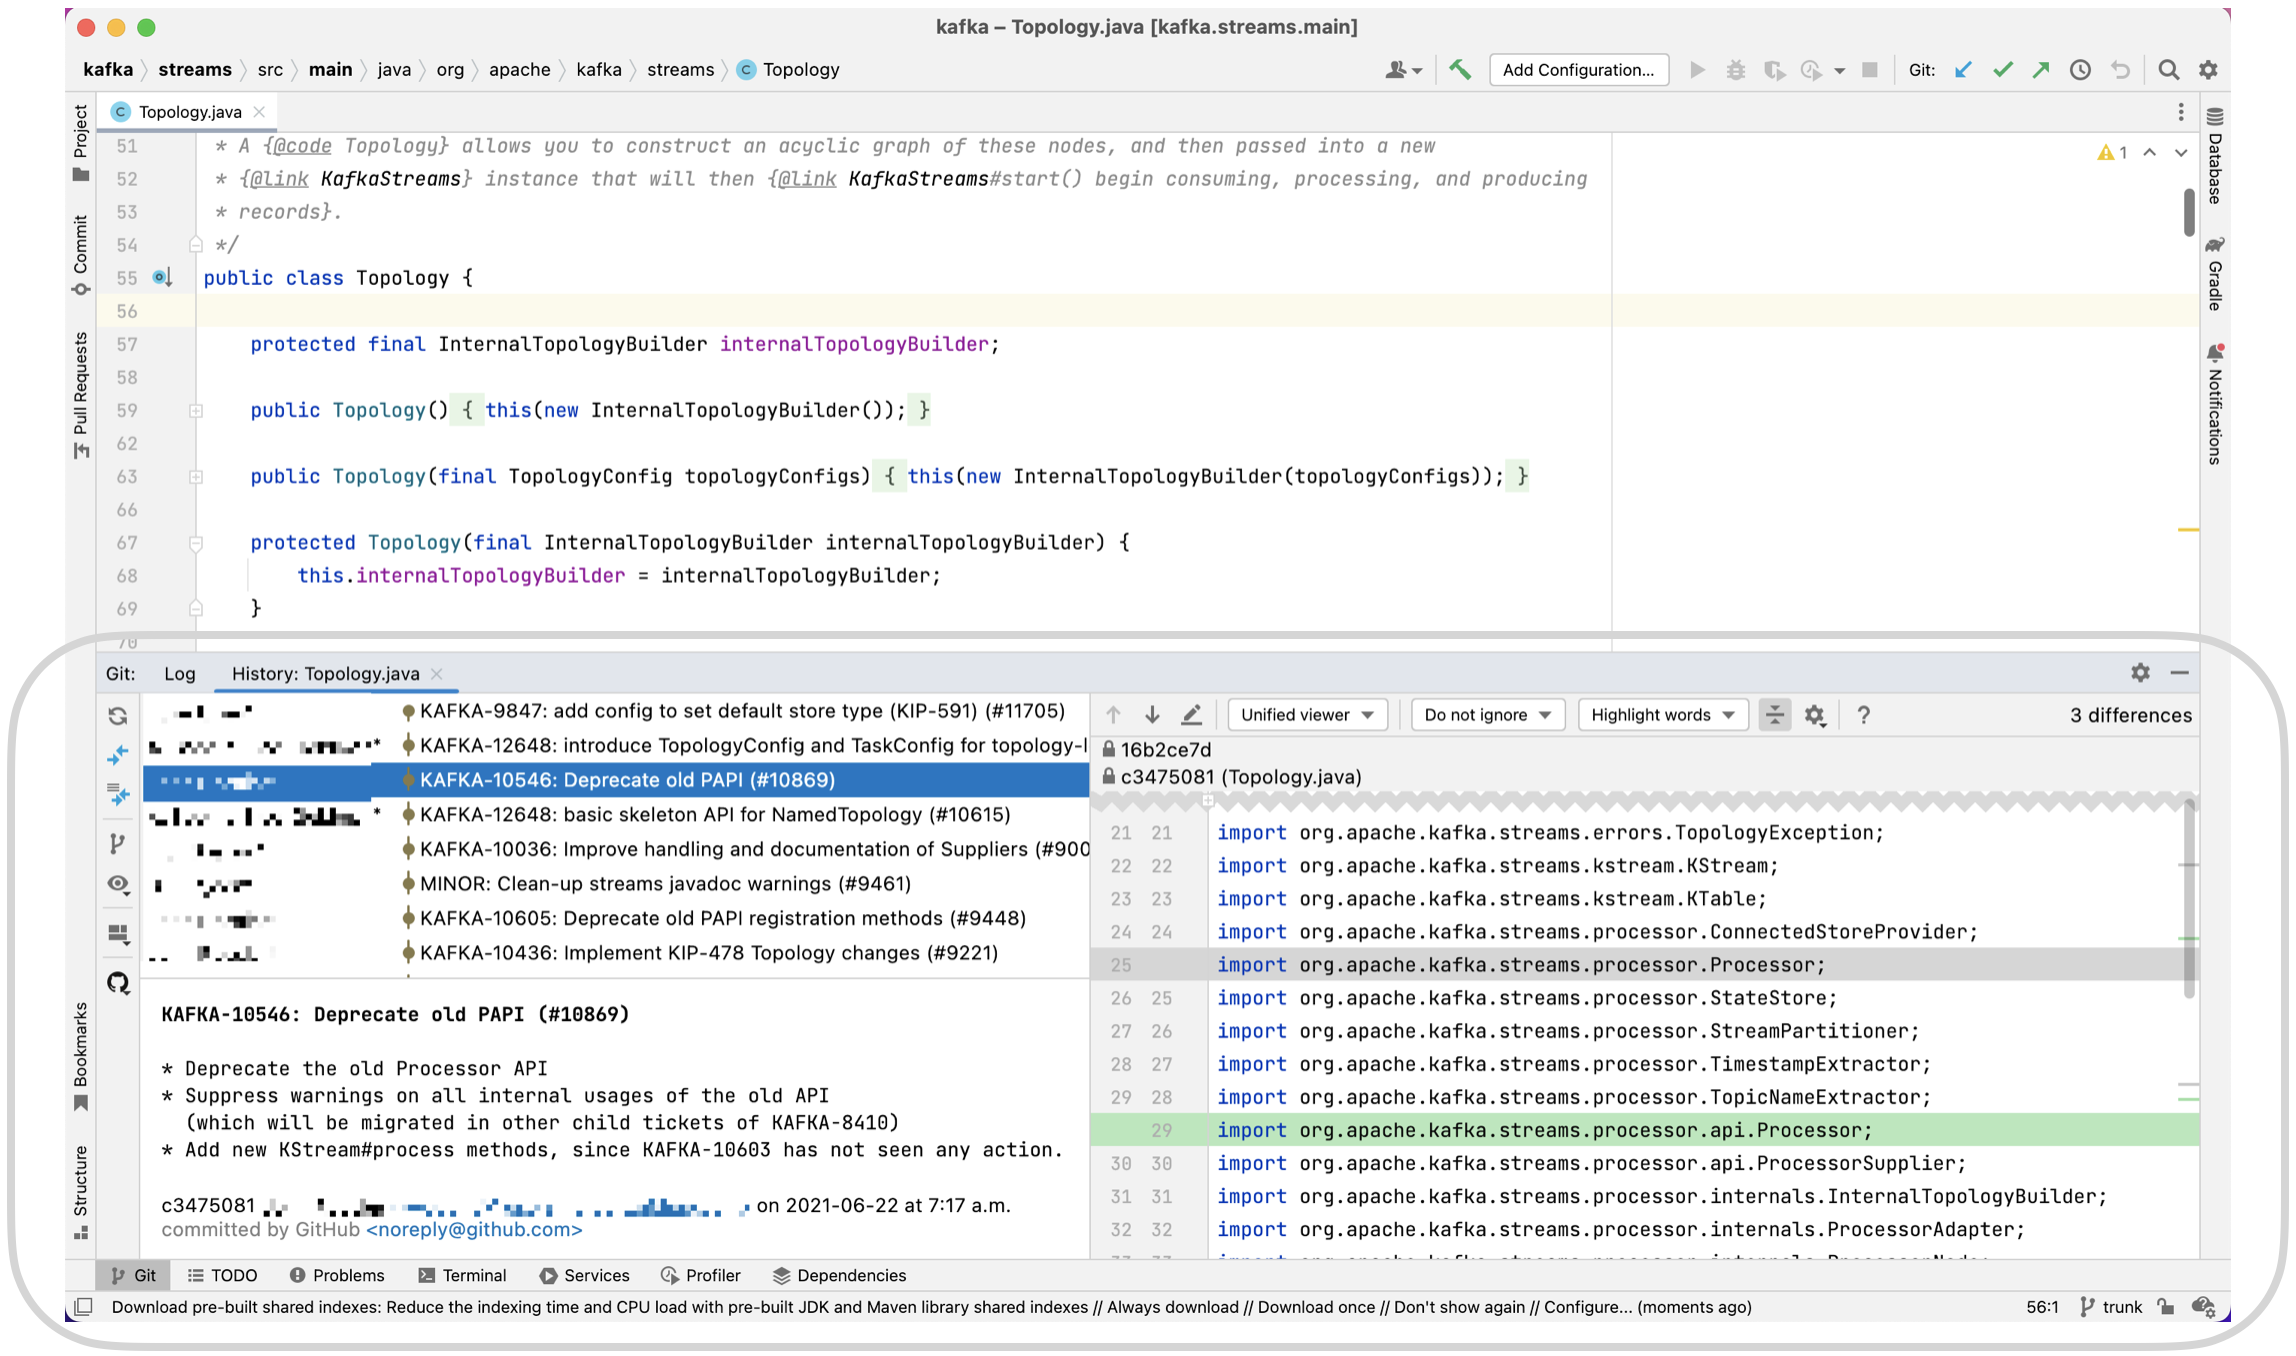
\includegraphics[width=\textwidth]{./images/intellij-overview.png}
    \caption{
        \rev{A capture of IntelliJ IDEA. 
        The revision history for the currently open \class{Topology} class 
        from Apache Kafka is visible in the bottom half tool window and circled in grey.
        Individuals' names and email addresses have been obfuscated.}
    }
    \label{fig:IntelliJ-Overview}
\end{figure}

We developed Intelligent History using the IntelliJ Platform \entity{SDK}.\footnote{\url{https://www.jetbrains.com/opensource/idea/}, verified 5/23/2022}
As a plugin, Intelligent History integrates with IntelliJ's ``Show History'' feature seamlessly as the plugin adds actions that can be invoked from a toolbar in IntelliJ's existing interface for exploring a file's commit history. 
This makes the features of Intelligent History complimentary to IntelliJ's existing version control interface.
We designed Intelligent History to support the following questions a developer might ask when searching for code rationale information in a file's revision history:

\begin{enumerate}[label={(\arabic*)}]
    \item \textit{Which commits are likely to be meaningful for understanding the decisions and choices involved in the evolution of this file?}
    \item \textit{Is there an interesting discussion or rationale that motivated the changes in a commit?}
\end{enumerate}

The features of Intelligent History are implemented as \emph{actions} in the IntelliJ Platform \entity{SDK} 
and are indicated in \autoref{fig:Intelligent-History-Overview}, 
where the actions are presented as icons in IntelliJ's \entity{VCS} file history tool bar.
Intelligent History has the following actions, also regarded as features, which the user can invoke:

\begin{itemize}
    \item[(\feature{1})] \textit{Highlight Important Changes}: 
        A toggleable action that automatically detects less important commits and applies highlighting on a file's commit history to visually distinguish potentially important commits from less important commits. 
        The determination of less important commits is based on a set of heuristics in the form regular expressions applied to the diff content of commits. 
        The implementation of this heuristics-checking approach is described further in \autoref{sec:Heuristics}. 
        \autoref{fig:Intelligent-History-A} demonstrates the highlighting action toggled on and applied to the commit history for a class.
    \item[(\feature{2})] \textit{Show Diff Metadata}: 
        An action that displays a pop-up summary of metadata information on the diff for a user-selected commit in a file's commit history. 
        This summary contains a categorization of code changes in a commit's diff content and the number of lines detected in a diff according to the heuristics used for determining less important commits. 
        This information is provided to raise the developer's confidence in Intelligent History's highlighting as the pop-up exposes the computed number of changes per category that Intelligent History uses for fading out certain commits in the file commit history. 
        The details of this categorization is also further explained in \autoref{sec:Heuristics}. \autoref{fig:Intelligent-History-B} shows an example of the metadata pop-up invoked for a selected commit.
    \item[(\feature{3})] \textit{Show Jira Issue}: 
        An action that extracts the Jira issue \entity{ID} for a user-selected commit in a file's commit history and fetches and displays the Jira issue information in a dedicated tool window. 
        The Jira issue ID is extracted from a commit's message using regular expressions. Along with the Jira issue information, 
        this action also provides a metadata summary of the Jira issue \rev{containing metrics that could indicate an issue as likely to contain rationale information as an
        important change or rationale information provided in the comments by a commit author or other project members. 
        The metadata} includes metrics on the number of comments on the Jira issue made by commit author, 
        the total number of comments on the Jira issue exluding bot comments, the total number of unique people involved in the Jira issue based on comments including the Jira issue assignee, 
        the number of people subscribed to the Jira issue (``watches''), the number of votes on the Jira issue, the number issue links, 
        and the number of sub-tasks. \autoref{fig:Intelligent-History-C} illustrates the tool window showing the information extracted for an automatically identified Jira \entity{ID} from a selected commit.
\end{itemize}

\begin{figure}
    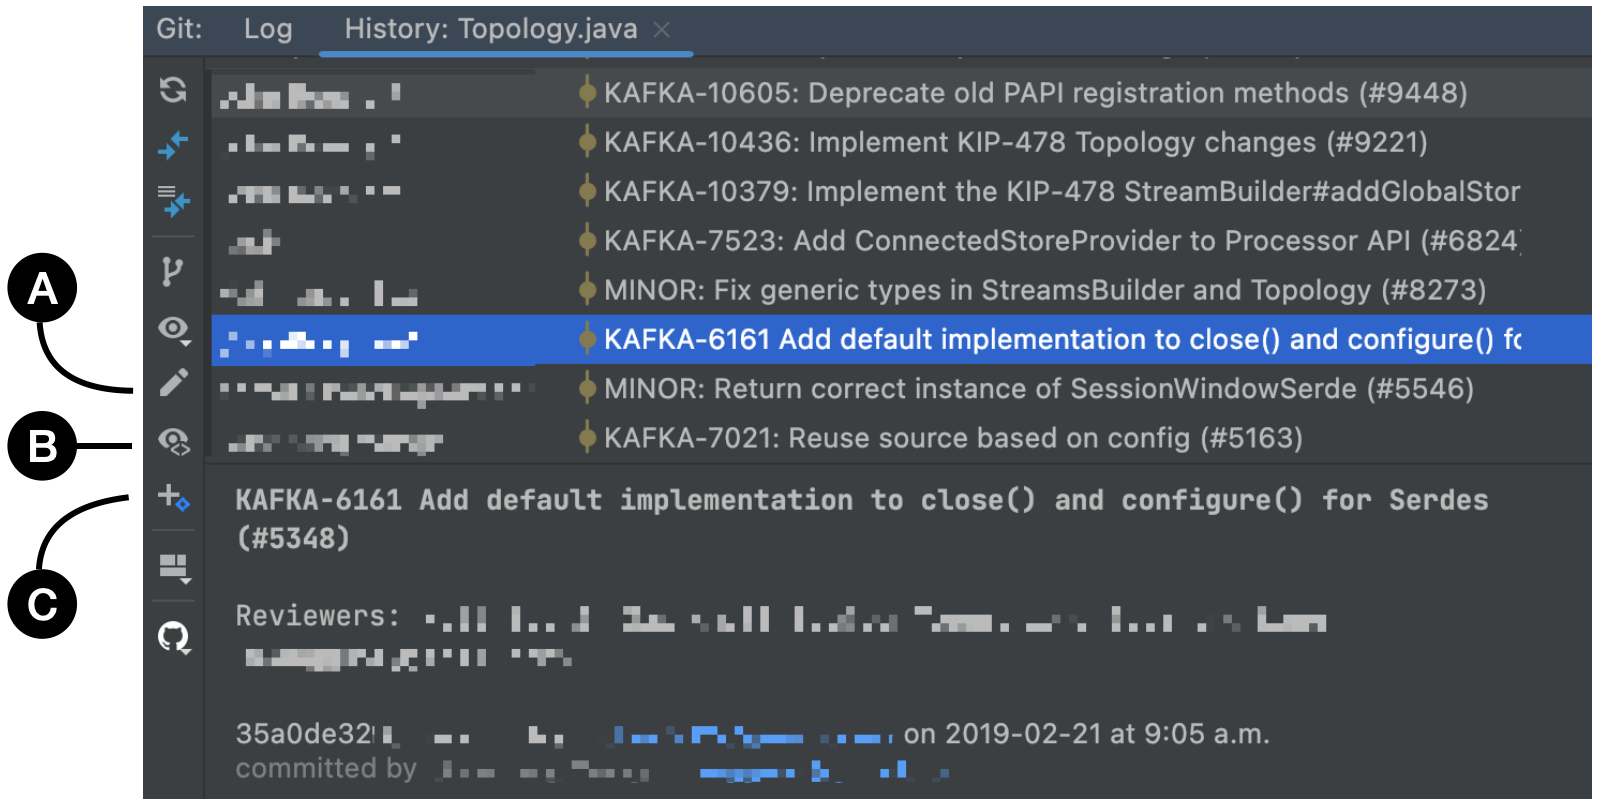
\includegraphics[width=\textwidth]{./images/intelligent-history-overview.png}
    \caption{
        Overview of the actions added by the Intelligent History plugin. 
        We use the following labels: (\feature{1}) \textit{Highlight Important Changes}; (\feature{2}) \textit{Show Diff Metadata}; and (\feature{3}) \textit{Show Jira Issue}.
    }
    \label{fig:Intelligent-History-Overview}
\end{figure}

\begin{figure}
    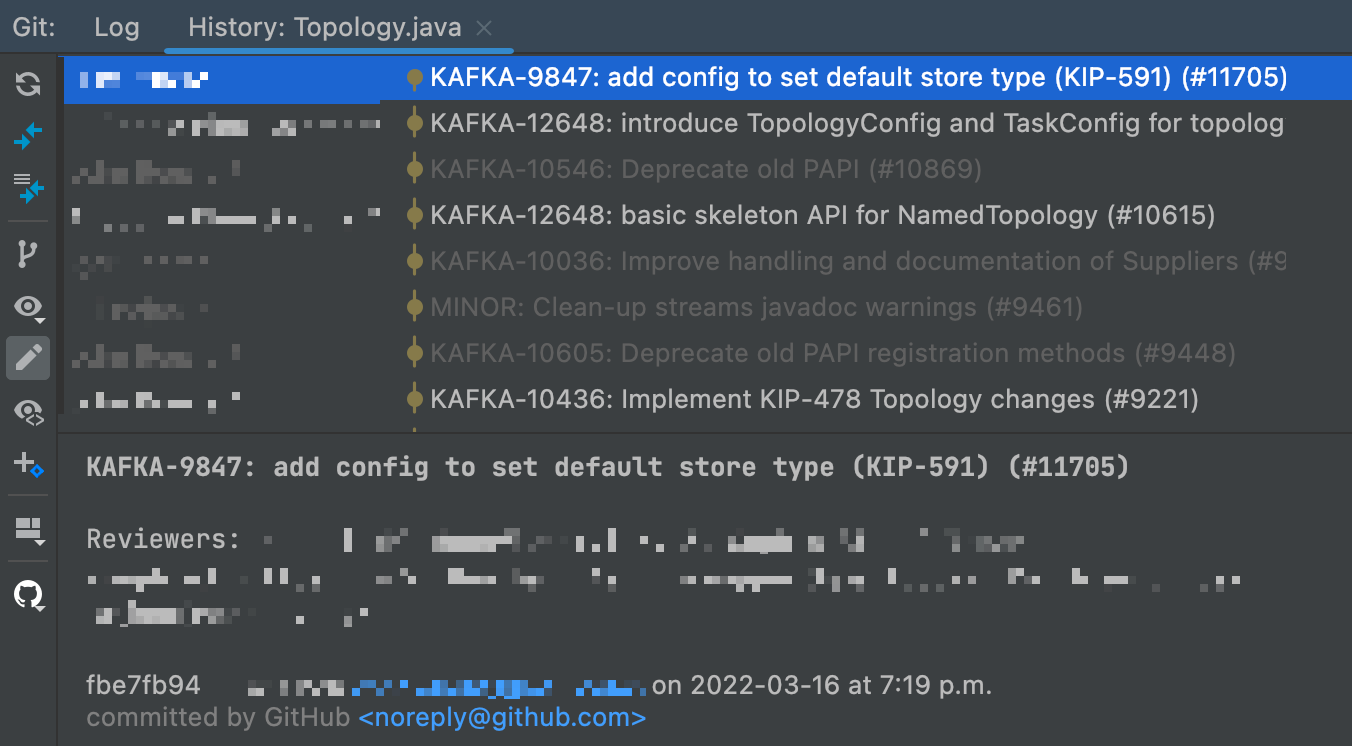
\includegraphics[width=\textwidth]{./images/intelligent-history-A.png}
    \caption{
        Feature (\feature{1}) \textit{Highlight Important Changes} of Intelligent History in the toggled on state. 
        Less important commits have been \rev{blended with} the foreground to make potentially more interesting commits stand out.
    }
    \label{fig:Intelligent-History-A}
\end{figure}

\begin{figure}
    \centering
    \subfloat[\centering Pop-up \label{subfig:Intelligent-History-B-Popup}]{{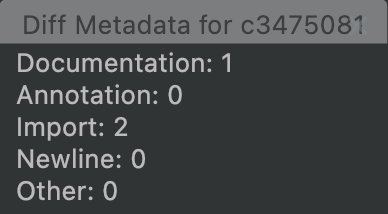
\includegraphics[width=4cm]{./images/intelligent-history-B-a.png}}}%
    \qquad
    \subfloat[\centering Diff \label{subfig:Intelligent-History-B-Diff}]{{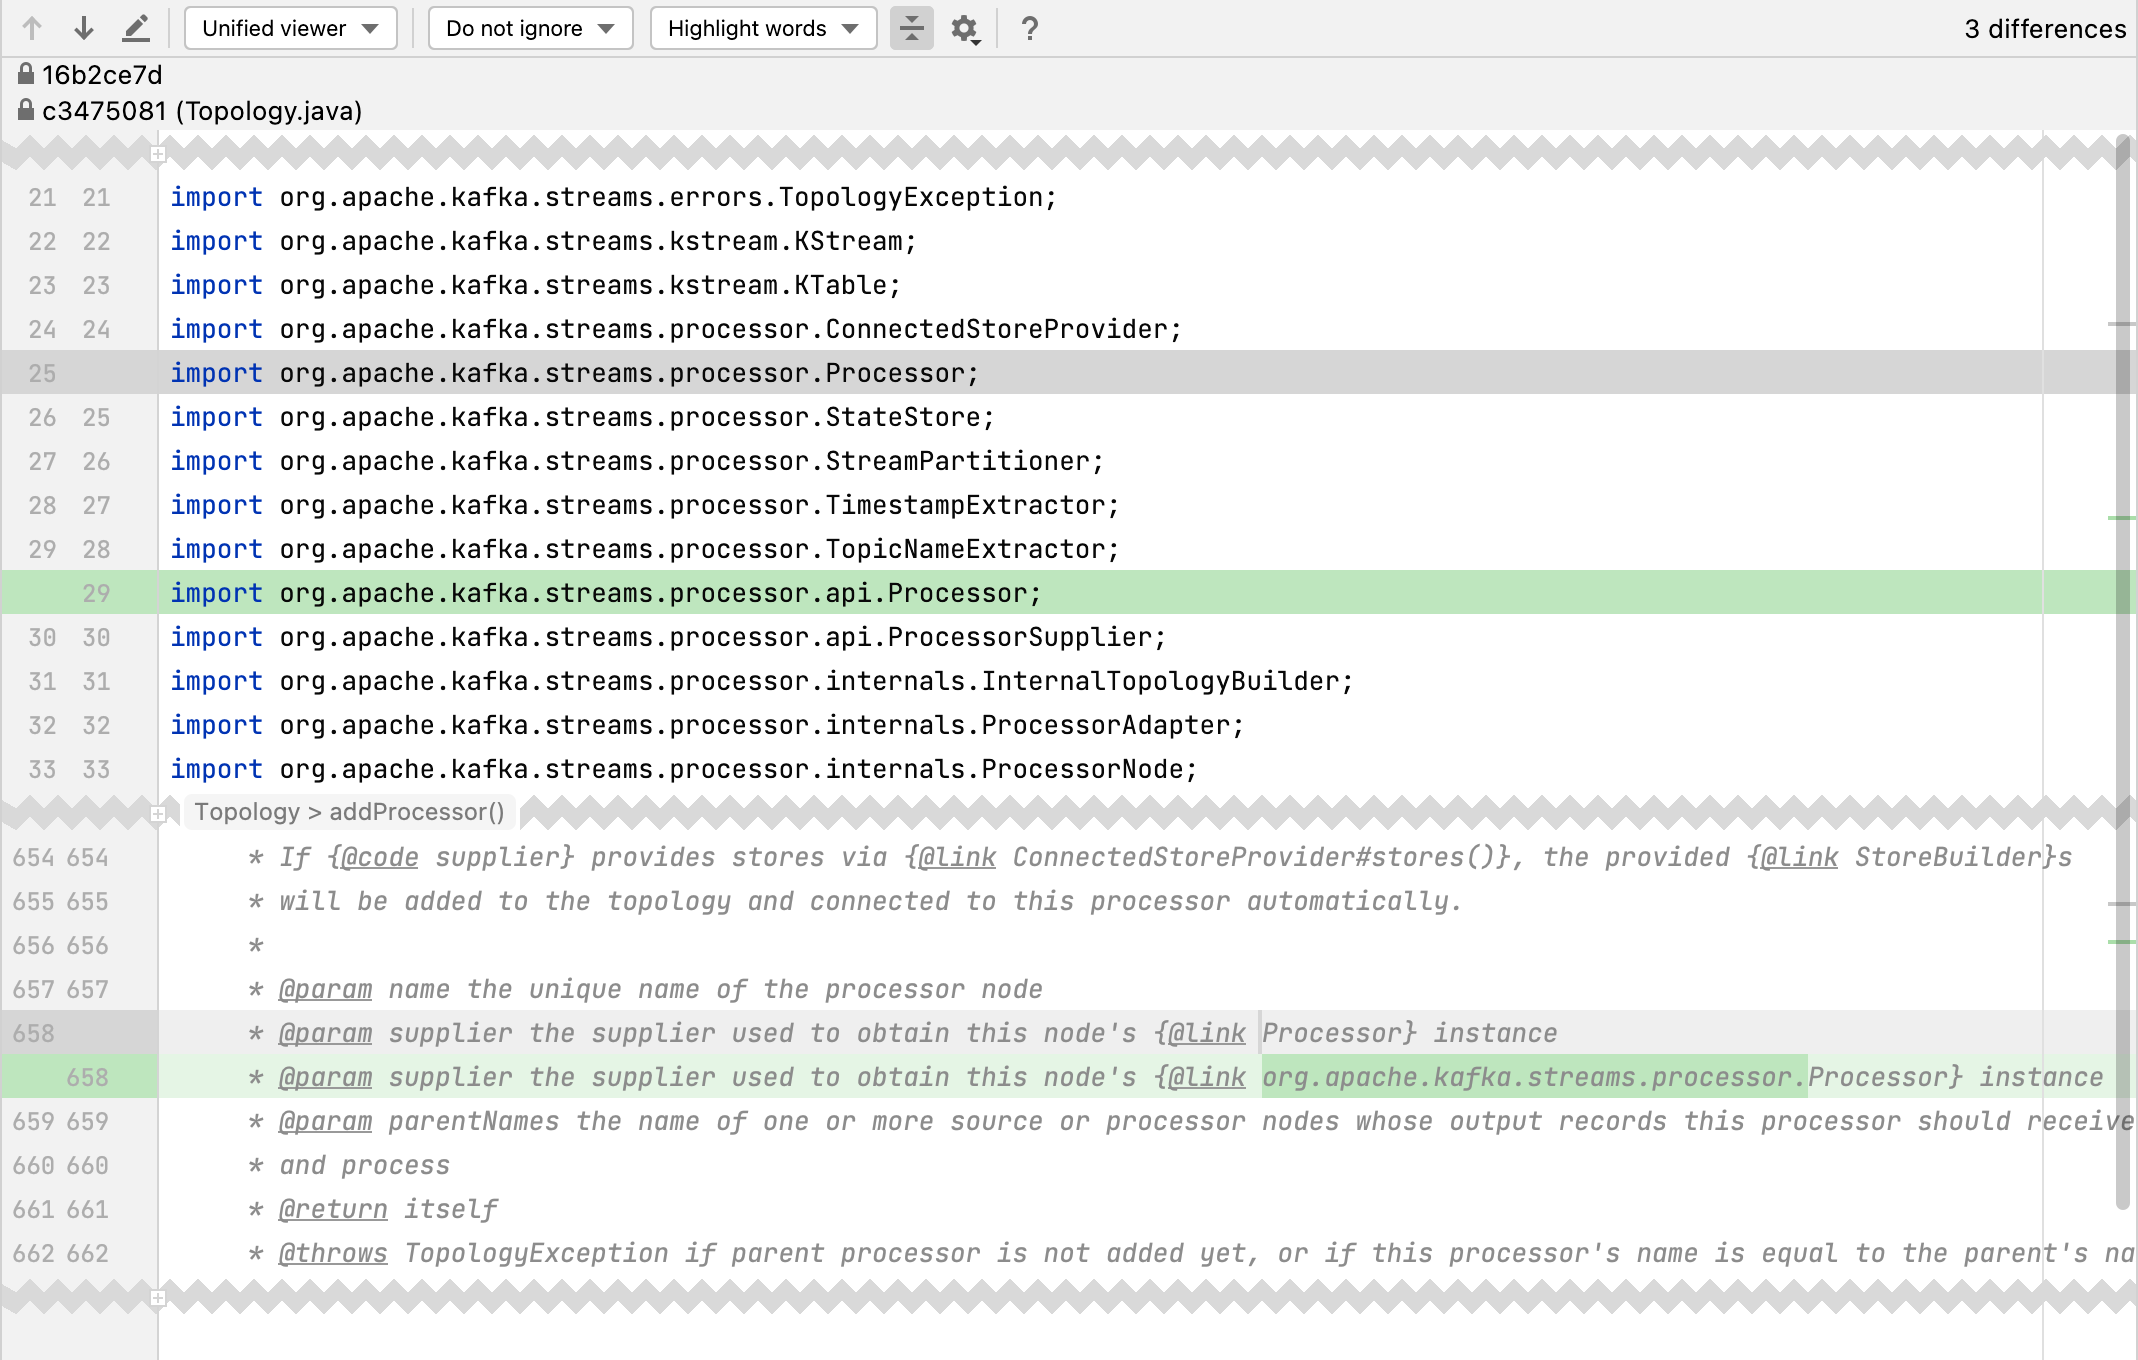
\includegraphics[width=12cm]{./images/intelligent-history-B-b.png}}}%
    \caption{
        Feature (\feature{2}) \textit{Show Diff Metadata} invoked on commit \commit{c3475081}. 
        The pop-up is shown in \autoref{subfig:Intelligent-History-B-Popup} 
        and displays the metadata for the diff in \autoref{subfig:Intelligent-History-B-Diff}.
    }
    \label{fig:Intelligent-History-B}%
\end{figure}

\begin{figure}
    \centering
    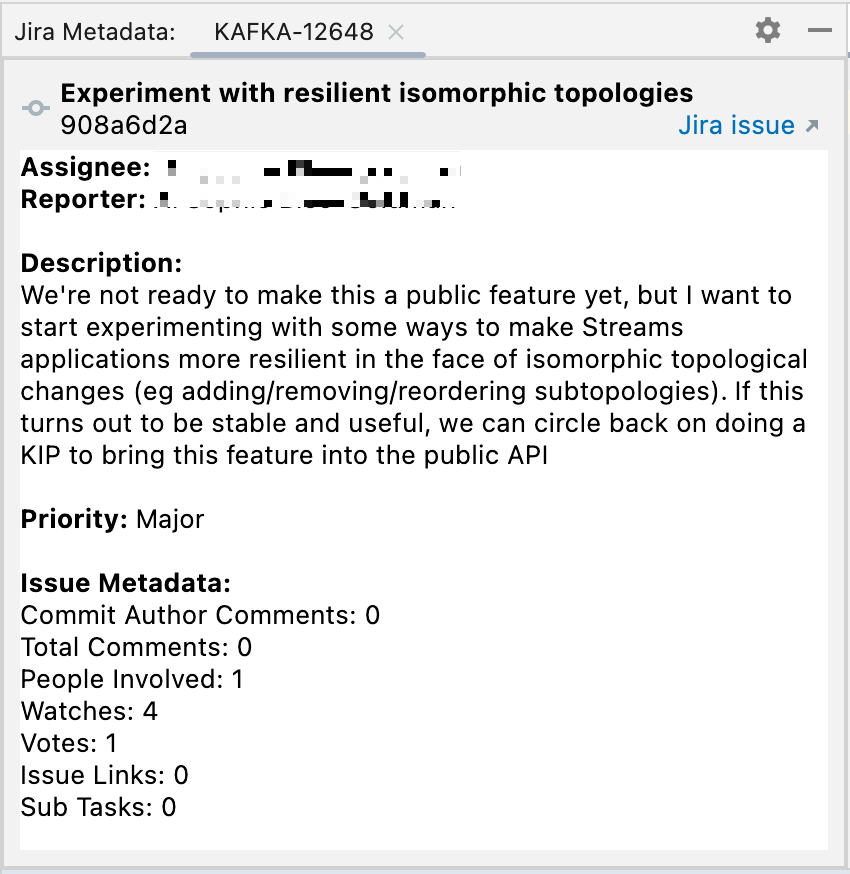
\includegraphics[width=7cm]{./images/intelligent-history-C.png}
    \caption{
        Feature (\feature{3}) \textit{Show Jira Issue} invoked on commit \commit{908a6d2a}.
        Shows the explicitly referenced Jira issue's title, assignee, reporter, description, priority, 
        and metadata in a tool window. A hyperlink to the Jira issue is also provided.
    }
    \label{fig:Intelligent-History-C}
\end{figure}

%%%%%%%%%%%%%%%%%%%%%%%%%%%%%%%%%%%%%%%%%%%%%%%%%%%%%%%%%%%%%%%%%%%%%%
\section{Heuristics for Analyzing Diffs}
\label{sec:Heuristics}

For distinguishing potentially important commits from trivial commits, 
we employ a heuristical approach based on empirical observation of file revision histories in the Apache Kafka project.
We identify patterns in the diffs of commits and categorize the \rev{commits} 
to determine less important or interesting commits in a file's revision history.
When referring to a commit's diff content, we mean the diff between the old version of a Java class in one commit, 
and the new version of the Java class after a commit has modified it.
This approach involves scanning the lines between commits for matches to a set of Java code patterns, 
which describe categories of trivial code changes.
Each pattern is expressed by a regular expression.

To assess the performance of our regular expression patterns, 
we apply them on two Java classes from the Apache Kafka repository and attempt to maximize coverage of the proportion of trivial commits.
We first manually identified the set of commits we considered trivial according to Kawrykow and Robillard's definition of non-essential changes \cite{kawrykow_non-essential_2011} and devised a set of categories, represented by regular expressions, to cover the patterns we observed in these lines of changes.
Recall in \autoref{fig:Topology-Commit-History}, the heuristics-based approach determines 41\% (9 out of 22) of the commits in the commit history for \class{Topology} to be less important.
For the commit history of \class{StreamsBuilder}, the heuristics-based approach detects 42\% (19 out of 45) of the commits from the commit history to be less important.
The diff metadata information for each commit in the commit history of \class{Topology} 
and \class{StreamsBuilder} are available \rev{in a public repository}.\footnote{\url{https://github.com/Alison-Li/ubcthesis-dataset}, verified 7/25/2022.}

While using heuristics for developing the regular expression patterns sacrifices some degree of accuracy on what is considered a non-essential or trivial line of code change to a user,
our heuristics as regular expression patterns have the advantage of being lightweight for efficiently analyzing diffs over other approaches to detecting code changes in programs, such as abstract syntax tree (\entity{AST}) matching and differencing techniques.
The categories of code changes expressed as regular exoressions also make the reasoning behind the highlighting of the commit history highly interpretable as the developer is shown why certain commits become faded with the highlighting.
Though the advantage of \entity{AST}-level granularity is that it produces edit scripts that directly refer to the structure of code, 
\entity{AST} matching and differencing techniques can have negative performance on runtime and memory consumption, 
which discouraged us from using them \cite{fluri_change_2007,pawlik_RTED_2011,falleri_fine-grained_2014}.
The goal of our approach is to understand if a minimal set of patterns for expressing trivial code changes can be effective at supporting a software developer in more efficiently navigating software history when searching for code rationale information.

Represented as regular expression patterns for the Java programming language, 
our approach for detecting trivial commits uses the following categories for a line of code that has been changed and presented as such in a diff: 

\begin{itemize}
    \item \textit{Documentation}: Changes that insert, delete, or modify lines representing Javadoc documentation and single-line or multi-line comments. We consider changes made to documentation in code as cosmetic.
    \item \textit{Annotation}: \sloppy Changes that insert, delete, or modify lines representing \code{@Deprecated} annotations or \code{@SuppressWarnings} annotations. The \code{@Deprecated} annotation indicates elements that should no longer be used but remain in source code to avoid breaking backward compatibility. We consider the marking of deprecated code as generally behaviour-preserving. The \code{@SuppressWarnings} annotation indicates named compiler warnings that should be hidden in the annotated element. We consider the marking of  suppressed elements as generally behaviour-preserving.
    \item \textit{Import}: Changes which involve the insertion, deletion, or modification of \code{import} statements. We consider these changes to be related refactoring, which is generally behaviour-preserving and unlikely to yield any further insight.
    \item \textit{Newline}: Changes involving the insertion or deletion of newlines. We consider these changes as behaviour-preserving and unlikely to yield any further insight.
    \item \textit{Other}: Any change not classified by the above categories. If a commit has a diff containing at least one change that is not classified by any of the above categories, then the commit is regarded as potentially interesting. Else, a commit is considered less interesting and will be presented as a faded out commit when the user invokes the \emph{Highlight Import Changes} action.
\end{itemize}

We use the \entity{java-diff-utils} \cite{java-diff-utils} library to extract the diff between two states of a file in the form of deltas. 
To obtain the state of a file for a given commit, we use the IntelliJ Platform's \entity{git4idea} library to retrieve the commits displayed in a file's commit history and the content of the file at the given commit.
The \entity{java-diff-utils} library provides a method that takes an old version $A$ and a new version $B$ of the contents of a file, represented as strings, and produces a list of \emph{abstract deltas} representing each change found from version $A$ to version $B$. 
Each delta contains a list of \emph{source lines} as strings and a list of \emph{target lines} as strings, where source lines represent consecutive lines in version $A$ and target lines represent consecutive lines in version $B$. 
For a set of consecutive lines that have changed from version $A$ to version $B$, a delta would contain the previous state of the lines in source lines and the new state of the lines in target lines.
For a delta that represents an insertion, the source lines would be empty, while the target lines would contain a list of the lines inserted in version $B$.
For a delta that represents a deletion, the target lines would be empty, while the source lines would contain a list of the lines deleted in version $B$.

For each commit in a file's commit history, beginning from the oldest commit to the most recent commit, 
we obtain the set of deltas for each sequential pair of commits.
Suppose we have a file $F$ and an ordered set of commits representing its commit history as 
$\{C_{1}, C_{2}, C_{3}, \dots, C_{n}\}$, where $C_{i}$ is a commit that affects $F$ and $i = 1, 2, 3, \dots, n$ denotes the oldest commit to the most recent commit in $F$'s commit history.
We use \entity{java-diff-utils} to obtain the diffs for the state of $F$ in the commit pairs 
$\{\varnothing, C_{1}\}$, $\{C_{1}, C_{2}\}$, $\{C_{2}, C_{3}\}$, \dots, $\{C_{n-1}, C_{n}\}$.
We compare an empty set, representing an empty string, with the state of $F$ in the first commit $C_{1}$ since the first commit in a file presumably introduces the file $F$ and its initial content.
For each pair of commits, we take the contents of file $F$ in each individual commit in a pair, obtain a list of deltas, and apply regular expression pattern matching on each string in a delta's list of source lines and list of target lines to count the number of lines that match a category.

This categorical information for a user-selected commit is exposed as \emph{diff metadata} in a pop-up when the user invokes the \textit{Show Diff Metadata} action provided by Intelligent History.
\autoref{subfig:Intelligent-History-B-Popup} illustrates the metadata information in a pop-up for the diff presented in \autoref{subfig:Intelligent-History-B-Diff}.
As shown in \autoref{subfig:Intelligent-History-B-Diff}, the commit \commit{16b2ce7d} for \class{Topology.java} consists of deleting an \code{import} statement, inserting an \code{import} statement, and the modification of a Javadoc comment.
Exposing this metadata to the user allows the user to obtain a summary about the lines changed from one commit to another commit and to also understand how Intelligent History highlights commits in a file's commit history.

%%%%%%%%%%%%%%%%%%%%%%%%%%%%%%%%%%%%%%%%%%%%%%%%%%%%%%%%%%%%%%%%%%%%%%
\section{Use Case}
\label{sec:Use-Case}

With the features of Intelligent History established in \autoref{sec:Implementation}, we describe how we anticipate a user might be able to use the actions from Intelligent History. 
In \autoref{sec:Implementation}, we outlined the three actions a user can invoke while examining a file's history using IntelliJ's built-in file revision history view: 
(\feature{1}) \textit{Highlight Important Changes}; 
(\feature{2}) \textit{Show Diff Metadata}; and 
(\feature{3}) \textit{Show Jira Issue}.

Suppose a developer who is new to the Apache Kafka project would like to obtain an 
overview of changes so far that have improved some functionality or usability of 
the \class{StreamsBuilder} class over time.
The commit history for \class{StreamsBuilder} contains a total of 45 commits.
Upon invoking feature (\feature{1}), 19 of the commits become faded in the commit history.
Further, the developer can select any commit from the commit history and call feature (\feature{2}) to understand how Intelligent History's highlighting has been applied on the \class{StreamsBuilder} commit history.
Browsing through the remaining 26 highlighted commits in the \class{StreamsBuilder} commit history, the developer can scan the messages of the commits to identify potentially interesting commit titles.
For any commits of interest that have a commit message prefixed with a Jira issue \entity{ID}, the developer can use (\feature{3}) to access a summary of the Jira issue information within their \entity{IDE}.

The Jira issues open in a separate tool window in IntelliJ as tabs to allow the developer to view several issues at a time and compare them.
The developer scans commit messages and the diffs for the 26 highlighted commits in the \code{StreamsBuilder} commit history.
Among these 26 commits that reference Jira issue, the developer wishes to locate commits that contain information about the motivation and design choices involved in the changes they see in the diff.
When a commit message is unsufficient for providing information about the rationale behind a commit, the developer invokes (\feature{3}).
On the first 4 highlighted commits in the commit history, the developer is able to skip needing to perform an in-depth investigation into the Jira issues for commits with empty or un-informative Jira issue descriptions since the developer can know this beforehand using without leaving the \entity{IDE} by invoking feature (\feature{3}) on each highlighted commit.

For the fifth commit in the history, the developer sees refactorings in the diff for commit \commit{f2b74aa1} with the message:

\begin{center}
    \jira{KAFKA-5873:}{add materialized overloads to StreamsBuilder} 
\end{center}

\noindent to the overloaded \code{table}, \code{globalTable}, and \code{addGlobalStore} methods in the \code{StreamsBuilder} class as the diff contains changes to their method signatures and bodies.
The developer reads the commit message: 
``Add overloads for `table' and `globalTable' that use `Materialized' '' 
and finds it lacking in terms of explaining why this was done.
The developer invokes (\feature{3}) and is able to obtain a reference to \entity{KIP}-182, 
a Kafka Improvement Proposal\footnote{Kafka Improvement Proposals (\entity{KIP}s) in the Apache Kafka project are documents intended to capture the thought process behind major features introduced and changes that impact the public Kafka \entity{API}s. 
\entity{KIPs} contain the following sections: Motivation, Proposed Change, New or Changed Public Interfaces, Migration Plan and Compatibility, and Rejected Alternatives.} stating the purpose of the change was to address the overall accumulation of heavy method overloading in the interfaces associated with the Kafka Streams Domain Specific Language (\entity{DSL}), 
making it harder for consumers of the \entity{API} who use a modern \entity{IDE} to discover the interfaces and hence, was a usability problem.

Similar to our illustration of the developer's process of finding and synthesizing information about the change history of \class{StreamsBuilder} through the first 5 commits of its commit history, the developer can continue to use this these features of Intelligent History on the rest of the highlighted commits to efficiently locate and access rationale information for changes over time.
The use of feature (\feature{1}) allows the developer to reduce the number of commits they would have to manually skim to check if the commit contains a meaningful change, while feature (\feature{2}) provides the developer with the option to retrieve a quick summary of how Intelligent History's highlighting approach to the file's commit history.
Finally, the developer can use feature (\feature{3}) on commits of interest to check if the Jira issue associated with the commit can further enrich a commit's message and diff without further explanation on the motivation and rationale behind a commit's changes.
Overall, the features of Intelligent History reduces the time it would take for a developer in this example to manually determine relevant commits and minimizes the switches the developer would need to make between their \entity{IDE} and browser to find and read the associated Jira issue.

%%%%%%%%%%%%%%%%%%%%%%%%%%%%%%%%%%%%%%%%%%%%%%%%%%%%%%%%%%%%%%%%%%%%%%
\endinput

Any text after an \endinput is ignored.
You could put scraps here or things in progress.